\section*{Stream API}
	\begin{itemize}[noitemsep]
		\item Definiere was gesucht ist, nicht wie
		\item Framework zur Sequenz von Collection-Operationen (häufig höherwertige Funktionen mit Lambdas als Argumente)
		\item Regeln:
		\begin{itemize}[noitemsep]
			\item keine Interferenz (Darf Collection nicht selbst abändern), z.b.: \texttt{filter(p -> people.add(p))}
			\item keine Seiteneffekte (keine Abh. zu äusseren änderbaren Variablen), z.b.: \texttt{map(p -> { globalCount++; return p; })}
		\end{itemize}
		\item braucht immer eine Terminaloperation am Schluss.
	\end{itemize}
	\subsection*{Beginn}
		Begonnen wird immer mit dem Aufruf von \texttt{stream()} bei Collection. Beispiel:
		\lstinputlisting{code/StreamAPI_begin.java}
	\subsection*{Method Chaining / fluent Interface}
		\begin{minipage}{15cm}
			\lstinputlisting{code/StreamAPI_MethodChaining.java}
			\centering Ist äquivalent zu $\downarrow$
			\lstinputlisting{code/StreamAPI_MethodChaining_analog.java}
		\end{minipage}
		\hspace*{0.5cm}
		\begin{minipage}{3.3cm}
			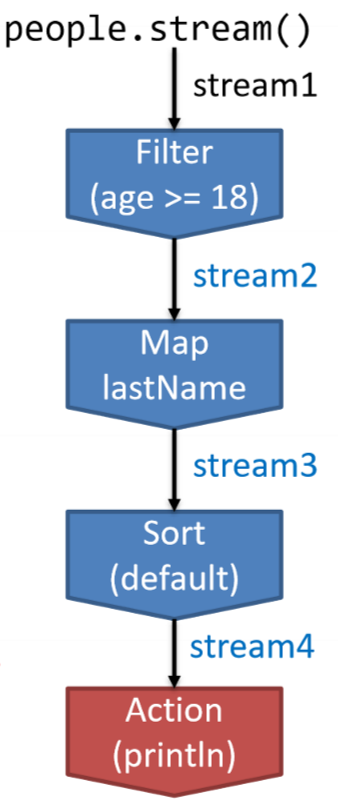
\includegraphics[width=0.8\columnwidth, right]{pics/StreamAPI.png}
		\end{minipage}
	\subsection*{Zwischenoperationen}
		\lstinputlisting{code/StreamAPI_Operations.java}
	\subsection*{Terminaloperationen} 
		\lstinputlisting{code/StreamAPI_Operations2.java}
	\begin{minipage}[t]{10cm}
		\subsection*{Endliche Quellen}
		\lstinputlisting{code/StreamAPI_sources.java}
	\end{minipage}
	\hspace*{0.5cm}
	\begin{minipage}[t]{8.3cm}
		\subsection*{Unendliche Quellen}
		\lstinputlisting{code/StreamAPI_sources2.java}
		Dies funktioniert, weil ein Element im Strom erst bereitgestellt wird, wenn der Nachfolger es wirklich anfordert. Als zweites Element kann zum Beispiel \texttt{.limit(1000)} folgen.
	\end{minipage}
	\subsection*{Rückumwandlungen}
		\begin{minipage}[t]{8.9cm}
			\lstinputlisting{code/StreamAPI_toArray.java}
		\end{minipage}
		\hspace*{0.5cm}
		\begin{minipage}[t]{8.9cm}
			\lstinputlisting{code/StreamAPI_toCollection.java}
		\end{minipage}
	\subsection*{Übersicht Collectors}
		\lstinputlisting{code/StreamAPI_Collectors.java}
	\subsection*{Gruppierungen}
	\lstinputlisting{code/StreamAPI_grouping.java}
	\lstinputlisting{code/StreamAPI_grouping2.java}	
